\section{Procedure e regole}
\label{procedure}
Nella seguente sezione sono riportate l'elenco di procedure e regole seguite dal gruppo \authorName{}.


\subsection{Avanzamento di un documento}
\label{avanzamenteo_doc}
Ogni qualvolta un redattore ritiene che la stesura di un documento sia terminata andrà seguita la seguente procedura (fig. \ref{proc_avanzamento}):
\begin{enumerate}
\item Il redattore dovrà contattare il \projectManager{} per informarlo della terminazione della redazione del documento;
\item Il \projectManager{} provvederà ad assegnare la verifica del documento ad uno dei \emph{Verificatori} disponibili che non sia in conflitto d'interessi;
\item Il \emph{Verificatore} provvederà alla verifica del documento;
\item Se sono stati trovati errori, il \emph{Verificatore} provvederà alla creazione di un ticket di correzione.
Successivamente il redattore correggerà gli errori trovati e infine si torna al passo uno;
\item Altrimenti il documento verrà approvato dal \projectManager{}.
\end{enumerate}
\begin{figure}[!h]
\centering
	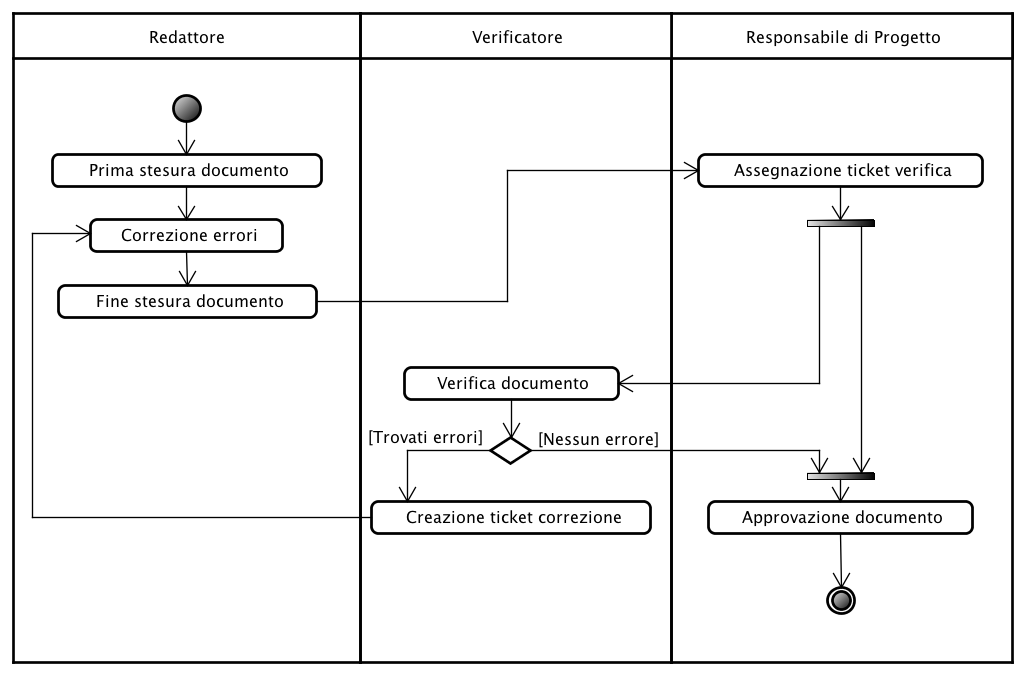
\includegraphics[height=10cm]{./content/Immagini/Avanzamento_Documento.png}
	\caption{Procedura di avanzamento di un documento}
	\label{proc_avanzamento}
\end{figure}

\subsection{Interazione con il repository}
\label{Interazione con il repository}
Per evitare conflitti nel repository, è \emph{indispensabile} eseguire le seguenti operazioni di sincronizzazione all'inizio e alla fine di ogni sessione di lavoro (fig. \ref{usorepo}):
\begin{enumerate}
\item \textbf{Pull:} prima di iniziare la sessione di lavoro, per ottenere i file aggiornati;
\item \textbf{Commit:} al termine di una sessione di lavoro, per commentare le modifiche effettuate;
\item \textbf{Pull:} subito prima di eseguire l'operazione di push;
\item \textbf{Push:} subito dopo l'operazione di pull, per caricare le modifiche nel repository\glossario{} remoto;
\item \textbf{Merge:} se durante l'operazione di push sorgono dei conflitti a seguito di modifiche effettuate da un altro membro.
\end{enumerate}
\begin{figure}[!h]
	\centering
	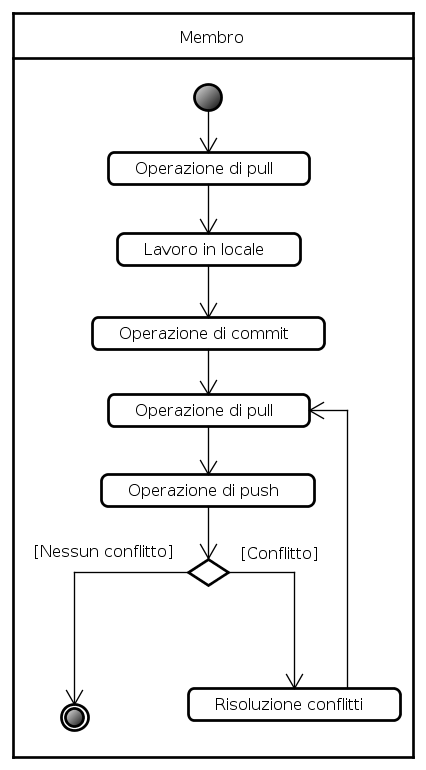
\includegraphics[height=10cm]{./content/Immagini/Utilizzo_Repository.png}
	\caption{Procedura per l'utilizzo del Repository}
	\label{usorepo}
\end{figure}
I commenti aggiunti al commit dopo la modifica di un file devono essere chiari e devono specificare le modifiche effettuate. Per garantire una buona leggibilità dei commenti, i commit devono essere effettuati per ogni file modificato o gruppo di files dello stesso contesto. Inoltre, per evitare conflitti, è \emph{sconsigliato} lavorare contemporaneamente sugli stessi file.

\subsection{Gestione del Glossario}
\label{gestione_gloss}

\subsubsection{Inserimento di un termine}
\label{inserimento_termine}
Per l'inserimento di un termine nel \emph{Glossario} si dovrà seguire la seguente procedura (fig. \ref{diagramma_add}):
\begin{enumerate}
\item Prima dell'inserimento di un termine andrà contattato il \projectManager{} per proporre l'inserimento del termine;
\item Solo nel caso in cui il \projectManager{} approvi l'inserimento del termine, esso andrà inserito nel \emph{Glossario} nell'ordine lessicografico corretto;
\item Successivamente all'inserimento, si dovrà provvedere a evidenziare ogni occorrenza del termine nei vari documenti.
\end{enumerate}
\pagebreak
\begin{figure}[!h]
 \centering
 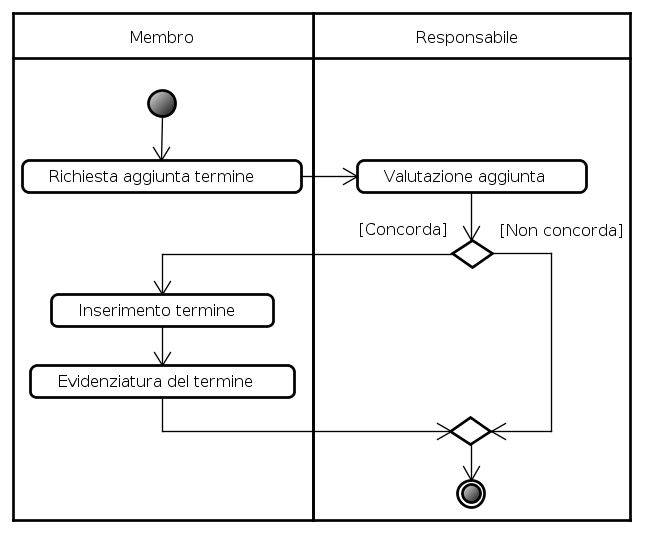
\includegraphics[height=10cm] {./content/Immagini/Aggiunta_Termine.png}
 \caption{Procedimento per l'inserimento di un termine.}
 \label{diagramma_add}
 \end{figure}

\subsubsection{Eliminazione di un termine}
\label{el_termini}
Ogni membro del gruppo per richiedere l'eliminazione di un termine del \emph{Glossario} dovrà seguire la seguente procedura (fig. \ref{proc_eliminazione}):
\begin{enumerate}
\item Dovrà essere contattato il \projectManager{} per proporre l'eliminazione;
\item Nel caso in cui il \projectManager{} approvi, il termine andrà cancellato dal \emph{Glossario};
\item Successivamente si provvederà a togliere tutte le marcature del termine, all'interno di tutti i documenti.
\end{enumerate}
\pagebreak
\begin{figure}[!h]
\centering
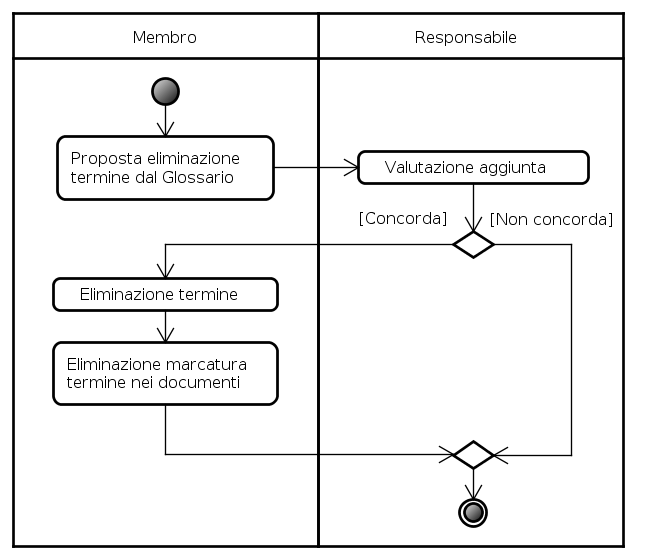
\includegraphics [height=10cm]{./content/Immagini/Eliminazione_Termine.png}
\caption{Procedimento per l'eliminazione di un termine}
\label{proc_eliminazione}
\end{figure}

\subsection{Rotazione dei ruoli}
\label{rotazioneruoli}
Durante lo svolgimento del progetto \project{}, è necessario che tutti i componenti del gruppo ricoprano tutti i vari ruoli definiti nel \PdP{}. Nel precedente documento verranno inoltre specificate le assegnazioni dei ruoli alle risorse, ripartite temporalmente e il quantitativo di ore che ciascuna risorsa dovrà svolgere in veste di un determinato ruolo.\\
Per pianificare l'impiego delle risorse in tale senso, il \projectManager{} si ispirerà alle seguenti regole:
\begin{itemize}
	\item Ogni risorsa dovrà ricoprire tutti i ruoli;
	\item Il carico di ore individuali dovrà essere equo.
\end{itemize}
Riportiamo di seguito le direttive che regolano l'assegnazione e la modalità di rotazione dei ruoli.\\
I ruoli verranno assegnati alle risorse in modo tale che cambino al termine di una macro-fase (vedi \PdP). Dato che i ruoli da ricoprire sono in quantità minore rispetto alle risorse, sarà necessario che una o più risorse ricoprano più ruoli durante la stessa macro-fase. Per regolamentare questa ulteriore rotazione, le risorse ricopriranno un singolo ruolo per settimana, ruotando tra i ruoli assegnati nella specifica macro-fase.\\
Ogni componente del gruppo potrà consultare, in qualsiasi momento, i diagrammi di Gantt\glossario{} che descrivono la gestione delle risorse e dei ruoli, in maniera tale che ognuno potrà sempre essere consapevole del ruolo ricoperto dagli altri componenti.